\section{Vision Transformer}\label{sec:vision-transformer}
In order to understand the paper \emph{Surgical-Dino} being examined in this report, it is crucial to first comprehend the algorithm used as the backbone of the suggested model: Vision Transformers (ViTs).
ViTs, as introduced by Dosovitskiy et al. in 2020~\cite{Dosovitskiy2020}, build on the work of Vaswani et al.~\cite{Vaswani2017}, adapting the transformer architecture for image classification, which until then was predominantly used for natural language processing (NLP). 
ViTs leverage the transformer's strengths in handling sequential data by splitting an image into a sequence of smaller patches, e.g., $16\times16$ pixels, and processing them through the transformer architecture as if they were tokens, as explained below.

The advantage of ViTs over conventional Convolutional Neural Networks (CNNs), which most previous state-of-the-art (SOTA) models for computer vision tasks were based on, lies in their ability to capture not only local features hierarchically but also global context information that may span different regions of the image~\cite{Khan2023}.
Additionally, they tend to scale better with the amount of data and parameters compared to popular CNN architectures but tend to perform worse when trained on smaller datasets from scratch~\cite{Han2023}.
The original transformer architecture, designed for machine translation, consists of an encoder-decoder structure that processes input sequences through an \emph{Embedding Layer}, \emph{Positional Encoding}, \emph{Encoder} containing \emph{attention heads} and \emph{MLPs}, a \emph{Decoder} and a \emph{prediction head}.
The following describes these components in the context of the original transformer architecture illustrated in Figure~\ref{fig:transformer}.
\begin{figure}[h!]
    \centering
    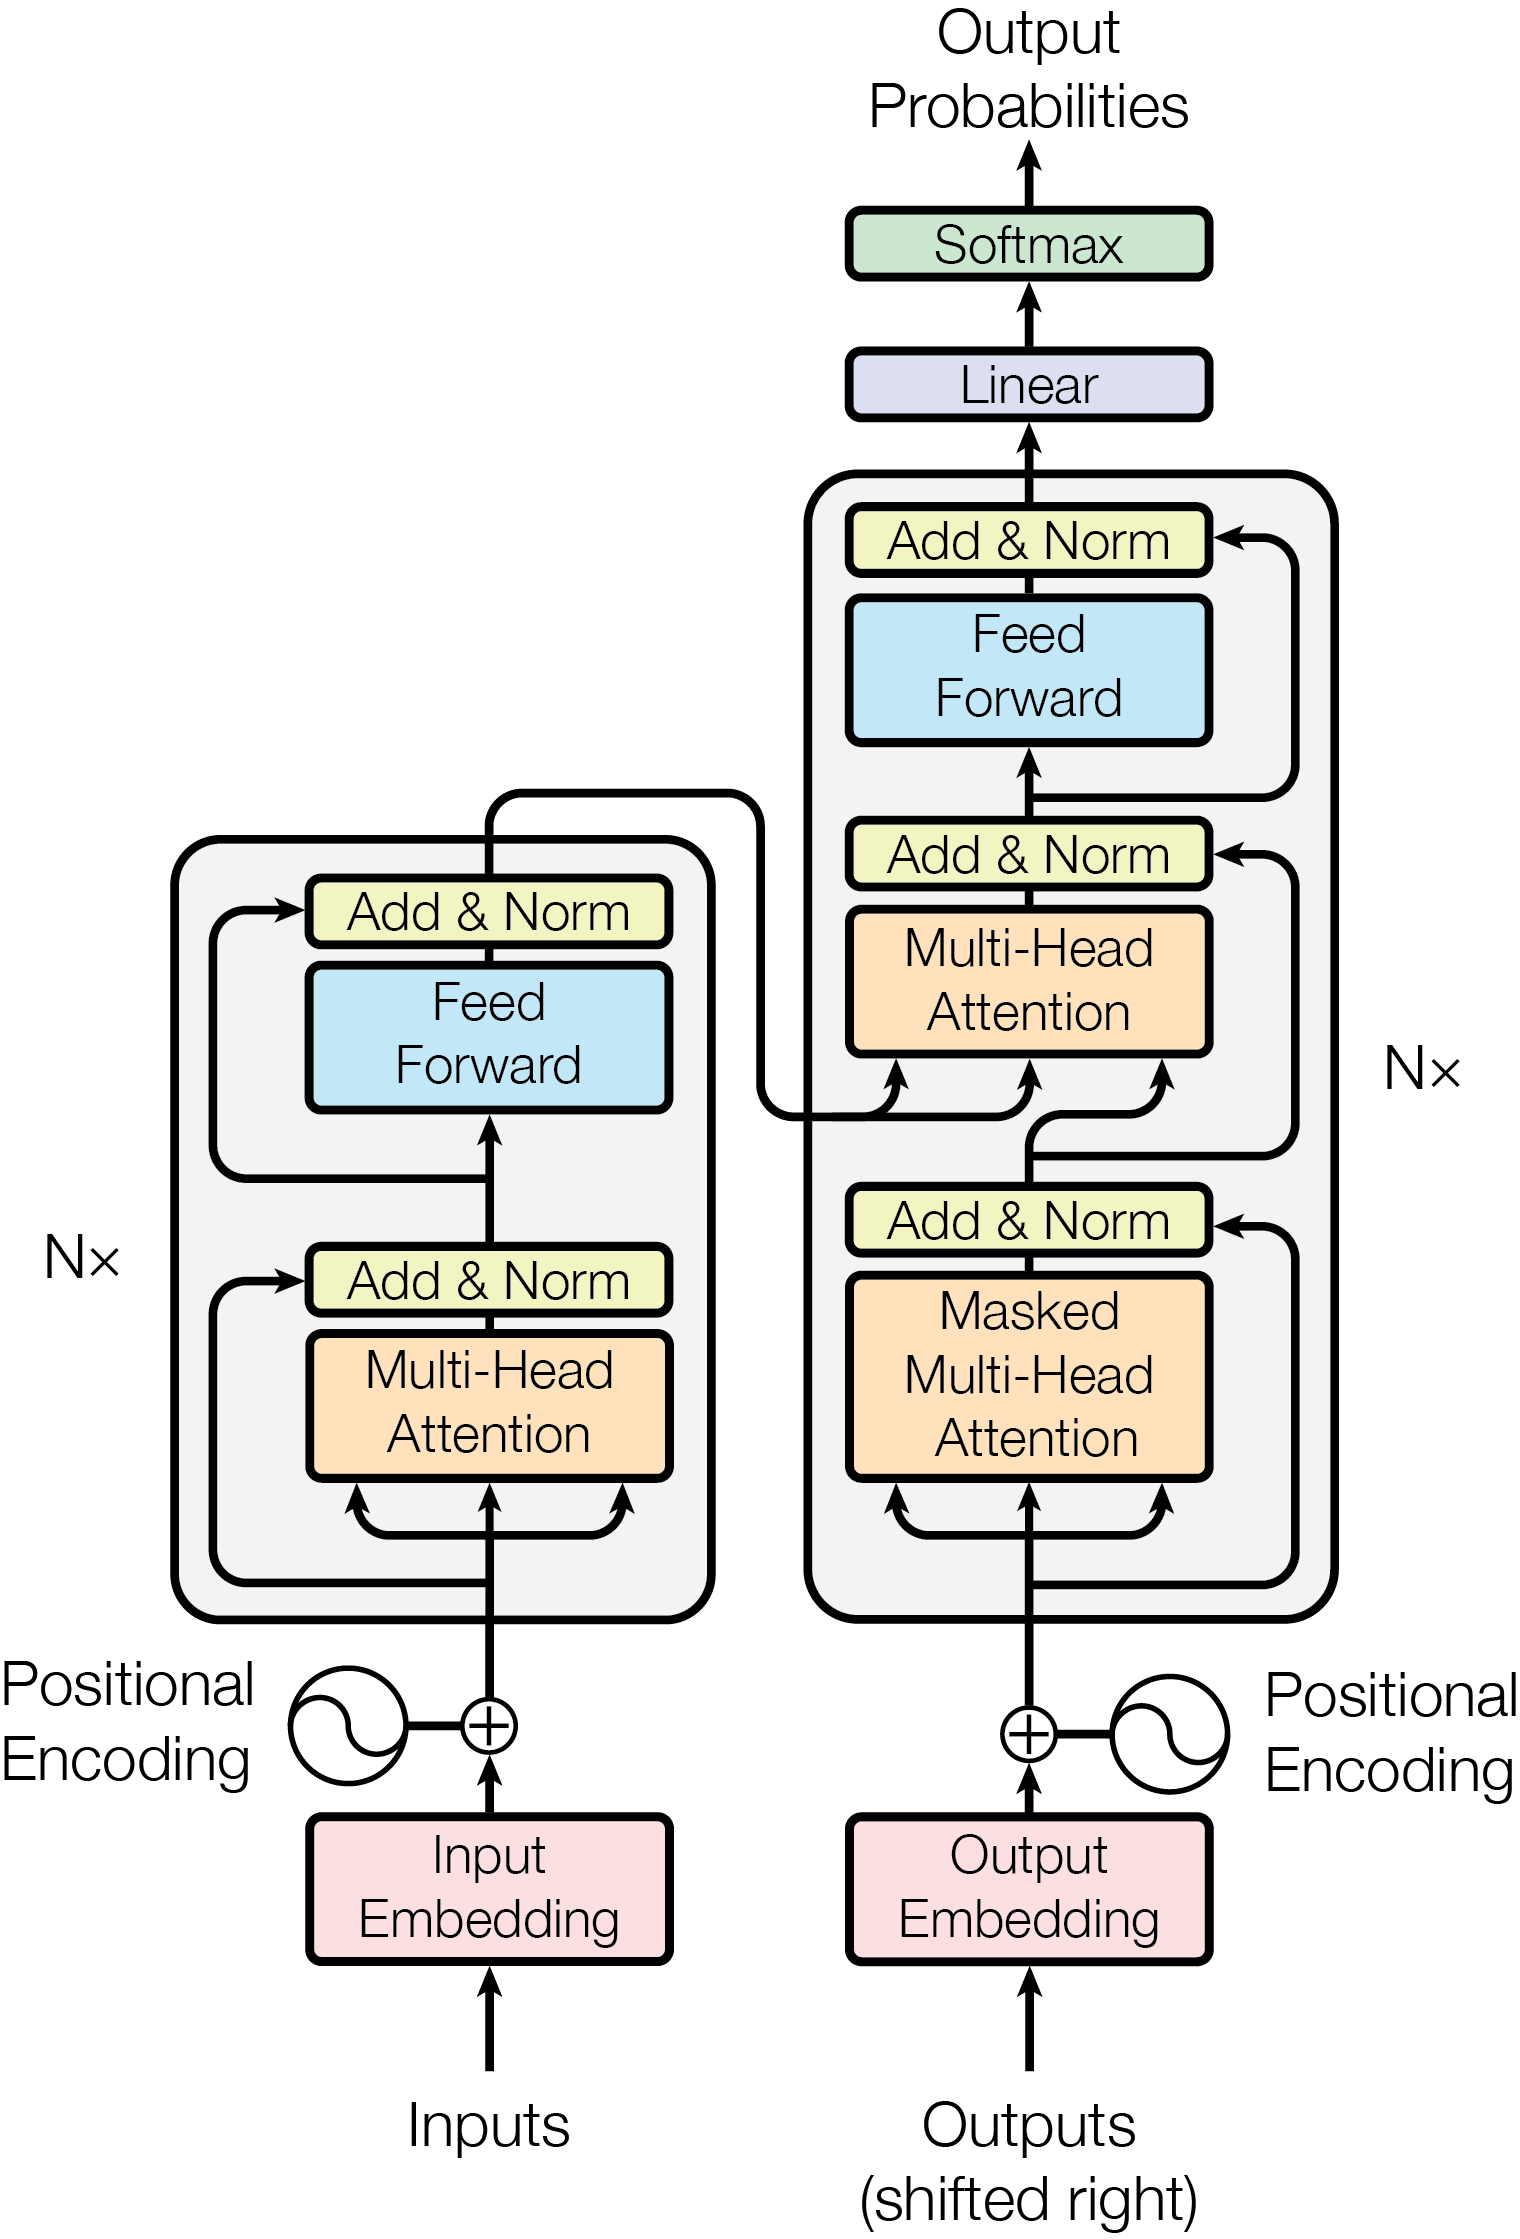
\includegraphics[width=0.3\textwidth]{images/TransformerArchitectureVaswani2017TransformerPage3.png}
    \caption[The original transformer architecture]{The transformer architecture (image from~\cite{Vaswani2017})}\label{fig:transformer}
\end{figure}

\textbf{Embedding Layer:} To ingest a sequence or an image into a transformer, it is first split into smaller pieces called tokens, which can be words, subwords and are then mapped into continuous vector representations with dimension $d_{model}$ called \emph{token vectors}.
The number of input tokens is denoted as $N$.
Vision transformer handles embedding slightly differnt creating tokens by splitting the images of dimension $\mathbb{R} ^{H \times W \times C}$ with $H$ being the height, $W$ the width and $C$ the number of channels into $N$ patches of dimension $\mathbb{R} ^{P \times P \times C}$ where $N = \frac{H \times W}{P^2}$.
Each patch then is flattened into an 1D vector and transformed to a length of $d_{\text{model}}$  using a linear layer resulting in the \emph{token vector}.
The trade-off is to split the sequence or image in as few parts as possible, which improves the inference of the model later on, while staying flexible enough for new unseen data, which is especially relevant for NLP tasks where often dictionaries are used to convert text to token vectors unlike ViTs where the data is already numeric and can directly be used as a token vector withouth a dictionary. 
These \emph{token vectors} form the columns of the \emph{Embedding Matrix} which, after the modification of the next step, will be the input of the \emph{Encoder}.

\textbf{Positional Encoding:} Following the embedding a \emph{positional encoding} is added to each \emph{token vector} in the \emph{Embedding Matrix}, which gives the model a hint of the order of the tokens in the sequence. 
This is needed as Transformers do not have an inductive bias about token order, unlike predecessors like Recurrent Neural Networks (RNNs)~\cite{Salehinejad2018} or Long Short-Term Memory (LSTM) networks~\cite{Hochreiter1997}.
The \emph{Positional Encoding} is usually either learned in form of a linear layer, or calculated using a fixed function such as the sine-cosine function as done for the original Transformer. 

\textbf{Encoder:} Typically an \emph{Encoder} consists of multiple \emph{Transformer Blocks} arranged sequentialy where on is build as described below: The \emph{Embedding Matrix} with the \emph{Positional Encoding} added, first is processed by a \emph{Multi-Head Attention} consisting of $h$ \emph{Attention Heads}.
The original paper achieved good results with $h=8$.
An Attention head first runs the \emph{Embedding Matrix} through three linear layers $W^Q, W^K\, \&\, W^V$ in parallel, producing three matrices: \emph{query matrix} $Q$, \emph{key matrix} $K$, and \emph{value matrix} $V$ each $\in \mathbb{R}^{d_{\text{model}\times d_k}}$ with $d_{\text{model}}$ defining the dimension the token vector is projected on to (512 in the original Transformer) and $d_k = \frac{d_{\text{model}}}{h}$ reducing the number of trainable parameters as it seams to be more parameter efficient to traine more attention heads with fewer parameters than fewer attention heads with more parameters.
These terms are analogous to database operations, where the query matrix is the search query, the key matrix is the database, and the value matrix is the data in the database.
This should convey the intuition behind the attention mechanism.
In \emph{Multi-Head Attention} the \emph{Embedding Matrix} is processed by several \emph{Attention Heads} in parallel to calculate the attention score using the Scaled Dot-Product Attention method as shown in Equation~\ref{eq:attention}. 
First the query matrix $Q$ and the transposed key matrix $K$ are multiplied, devided by the square of the dimension of the matrices $d_k$, to increase the gradients of the softmax function, and then scaled using softmax to a range of $0-1$.
This dot product is the \emph{Attention Matrix} of dimension $\mathbb{R}^{N^2}$ which contains the \emph{Attention Scores} of each token relating, or attending, to each other which can be interpreted as probabilities of how much a certain token is correlated to another token~\cite{Han2023}. 
This \emph{Attention Matrix} is then multiplied with the value matrix $V$ resulting in the weighted value matrix.
Having $h$ attention heads leads to $h$ weighted value matrices which get concatenated and processed by a final linear layer $W^O \in \mathrm{R}^{hd_k \times d_{\text{model}}}$ which transformes the outputs back to the dimension of the \emph{Embedding Matrix}.
This transformed \emph{Embedding Matrix} then is added to the unmodified input of the Transformer Block, which is called the \emph{Skip Connection}.     
\begin{equation}
    \text{Attention}(Q, K, V) = \text{softmax}\left(\frac{QK^{T}}{\sqrt{d_{k}}}\right)V
    \label{eq:attention}
\end{equation}

\textbf{Decoder:} The original Transformer architecture includes an decoder block which iterativley generates the output sequence token by token. While both encoder and decoder consist of the same building blocks, the decoder uses a masked multi-headed attention mechanism, zeroing out the lower left triangle of the \emph{Attention Matrix} containing the \emph{Attention Scores} to prevent the model from attending to future tokens. 
Following that a multi-head cross attention is applied connecting the output of the encoder with the decoder.
Since then works such as the BERT framework by Devlin et al.~\cite{Devlin2018} have shown that the decoder is not inherently needed for tasks like language translation, or text generation allowing for a simplified \emph{Encoder Transformer} architecture which is also used in ViTs.

\textbf{Prediction Head:}
Following the \emph{Encoder} and \emph{Decoder} blocks usually a MLP or CNN follows to processe the transformed \emph{Embedding Matrix} depending whether the task is a classification, regression or generation task.
For classification and regression the prediciton heads often only process one or more specific tokens, either the last sequence token as in the original transformer, or a prepending class token as done in the ViT or BERT architectures.
For generative ViTs such as ones used for depth estimation, use the whole \emph{Embedding Matrix}, sometimes even from different transformer blocks, to generate the output\cite{Cui2024}.

A compact summary of differences between the Transformer and ViT architecure can be seen in the Appendix~\ref{app:CompViT}.

Using this simplified Transformer architecture, as visualized in Figure~\ref{fig:vit}, ViTs have demonstrated superior performance over state-of-the-art convolutional neural networks (CNNs) in several image classification tasks~\cite{Mauricio2023}. 
Since the original ViT paper, transformers have found numerous applications in the computer vision field beyond image classification. 
For example, ViTs have been successfully applied in anomaly detection to identify unusual patterns in manufacturing images, and in medical imaging for monocular depth estimation in endoscopy~\cite{Ranftl2021}. 
These applications benefit from ViTs' ability to analyze the global context of images, and their performance is validated in diverse domains~\cite{Jamil2023}.
Although initially requiring significantly more training data than CNNs when trained from scratch, ViTs match or surpass state-of-the-art performance when finetuned, highlighting the potential of pre-training on large datasets and the flexibility of transformers in processing different types of data.

% Using this simplified Transformer architecture, as visualized in Figure~\ref{fig:vit}, ViTs have demonstrated superior performance over state-of-the-art convolutional neural networks (CNNs) in several image classification tasks~\cite{Mauricio2023}. 
% Since the original ViT paper, many more use cases beyond image classification have emerged for transformers in the computer vision field. 
% For example, ViTs have been successfully applied in various domains, including anomaly detection, where they identify unusual patterns in manufacturing images, and in medical imaging~\cite{Ranftl2021} for monocular depth estimation in the endoscopy domain. 
% These applications benefit from ViTs' ability to analyze the global context of images, demonstrating their potential in diverse and critical domains~\cite{Jamil2023}.
% Despite initially requiring significantly more training data than previous state-of-the-art CNN architectures when trained from scratch, ViTs effectively leverage the transformer architecture to match or surpass the previous state-of-the-art when finetuned, highlighting the importance of pre-training on large datasets and the flexibility of transformers in processing different types of data beyond natural language.
\begin{figure}
    \centering
    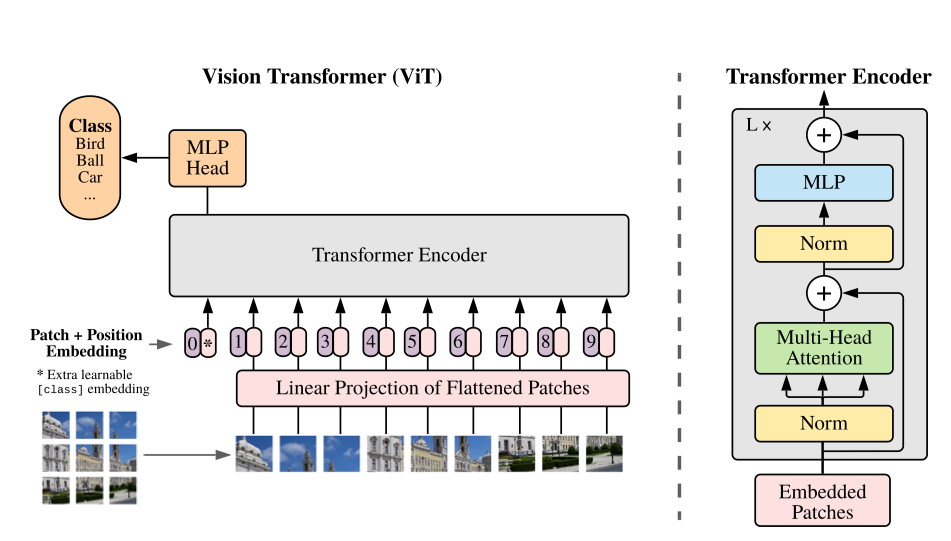
\includegraphics[width=0.8\textwidth]{images/vit_overview.png}
    \caption[The Vision Transformer architecture]{The Vision Transformer architecture (copied from~\cite{Dosovitskiy2020}).}\label{fig:vit}
\end{figure}

\section{Unsupervised Pretraining}\label{sec:unsupervised-pretraining}
\TS{This Section is undergoing corrections}
Now that ViTs allow for the creation of large-scale models for computer vision tasks, the need arises to train these models in an unsupervised manner to achieve even better performance by using even larger datasets without any lables.
Unsupervised learning involves training a network without any labels for the data, which facilitates the creation of huge datasets with millions or even billions of samples.
While these models often already show impressive results using clustering algorithms such as k-nearest-neighbor (KNN) clustering, they usually exhibit significant improvements when fine-tuned in a supervised manner for different downstream tasks, even when using small datasets and with limited computational resources available.
The overall term for these general models is foundation models~\cite{Bommasani2021}.
For NLP tasks, unsupervised approaches such as masked language modeling, as used in BERT~\cite{Devlin2018}, or generative pretraining, as used in GPT~\cite{Radford2018}, have been successfully applied.
While there are some works utilizing the same idea of predicting the next token, or a missing token, for computer vision tasks~\cite{Wei2022, Bao2021} there are alternative approaches tending to yield even better results.

% One of alternative approach among others was made popular by Hadsell et al.~\cite{Hadsell2006} and is called contrastive learning, using siemese networks consisting of two identical networks in parallel, to learn to differentiate between similar and different images. 
% The task to predict if the images both networks were presented with are similar, or different is called a contrastive task and is needed to prevent model collaps to a trivial solution, if the train task would be to predict the output of the other network given the same input.
% This was idea was develpoed further by Chen et al.~\cite{Chen2020} in 2020 who applied contrastive learning to a ResNet50 Network.

One alternative approach that has gained popularity is contrastive learning, as proposed by Hadsell et al.~\cite{Hadsell2006}, using siamese networks consisting of two identical networks in parallel to learn to differentiate between similar and different images.
The task of predicting whether the images presented to both networks are similar or different is called a contrastive task and is needed to prevent model collapse to a trivial solution, which would occur if the training task were to predict the output of the other network always given the same input.
This idea was further developed by Chen et al.~\cite{Chen2020} in 2020, who successfully applied contrastive learning to a ResNet50 Network improving its accuracy on the ImageNet-2012 Dataset with over $10\,000$ classes to almost $86\%$ being within the top-5 models at the time.

Grill et al.~\cite{Grill2020} then introduced the Bootstrap Your Own Latent (BYOL) framework eliminating the need for negative samples to prevent model collaps by changing the way both networks udpate their weights. 
Grill et al. figured, it, to prevent model collaps, they would randomly initialize the second network, the teacher network, and freeze its weights, the student network would still while not achieving good results in down stream tasks, definitly learns meaninfull representations of the images.
To further improve this they figured that updating the teacher weights based on the moving average of the student weights would prevent the model from collapsing to a trivial solution.
This however is yet to be mathematically proven, but the authors empirically show, that the model does not collaps and intentionally made designchoices to prevent that.\textbf{dig into the reasoning they give in the paper}

Grill et al.~\cite{Grill2020} then introduced the Bootstrap Your Own Latent (BYOL) framework, eliminating the need for negative samples needed for contrastive learning, to prevent model collapse by changing the way both networks update their weights.
Grill et al. found that randomly initializing the second network, the teacher network, and freezing its weights and only updating the student networks weights during training already led the student network to learn meaningful representations of the images.
The student network, while not achieving high accuracies in classification tasks, still learned meaningful representations of the images.
To further improve this, they found that updating the teacher weights based on the moving average of the student weights, instead of using backpropagation would prevent the model from collapsing to a trivial solution.
This has yet to be mathematically proven, but the authors empirically show that the model does not collapse which was veryfied by numerouse works\TS{Add references}.

The pipeline of BYOL starts with generating several augmented crops and providing each network, the student and teacher network, with a different random augmentation of the same image.
Next, both networks process their input inside a ViT encoder, called the representation block.
This is followed by a few MLPs for dimensionality reduction.
The student network also has another prediction MLP at the end, which introduces asymmetry into the model, likely making the trivial solution of outputting a constant vector less likely.
Afterward, a scaled cosine similarity between the output of the student network $q_{\theta}(z_{\theta})$ and the teacher network $\bar{z}'_{\xi}$ is calculated as shown in Equation~\ref{eq:byolloss}.
Then, the inputs of the networks are switched, so both networks get the images of the other one.
The cosine similarity is again calculated, and the loss is calculated as the sum of both similarities and used to optimize the student network's weights.
The weights of the teacher network $\xi$ are updated as the exponential moving average of the student network's weights $\theta$ as shown in Equation~\ref{eq:byol}, with $\tau$ set to 0.99 in the BYOL paper.
After training the representation block inside the student network can be used for downstream tasks.
\begin{equation}
    \mathcal{L}_{\theta, \xi} \triangleq \left\| \bar{q}_{\theta}(z_{\theta}) - \bar{z}'_{\xi} \right\|_2^2 = 2 - 2 \cdot \frac{\langle q_{\theta}(z_{\theta}), z'_{\xi} \rangle}{\| q_{\theta}(z_{\theta}) \|_2 \cdot \| z'_{\xi} \|_2}\label{eq:byolloss}
\end{equation}
\begin{equation}
    \xi \leftarrow \tau \xi + (1-\tau) \theta
    \label{eq:byol}
\end{equation}

\section{DINO: Unsupervised Learning with Vision Transformers}\label{sec:dino}
\TS{This Section is undergoing corrections}
\begin{figure}
    \centering
    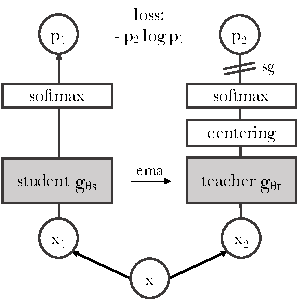
\includegraphics[width=0.5\textwidth]{dino_arch.pdf}
    \caption[The DINOv1 Architecture]{The DINOv1 Architecture showing the Student-Teacher Setup. \emph{sg} stands for stop gradient (image from~\cite{Caron2021})}\label{fig:dinov1}
\end{figure}

The \textbf{DI}stillation with \textbf{NO} labels (DINO) framework, introduced by Caron et al. in 2021~\cite{Caron2021}, is an approach for implementing self-distillation for Vision Transformers (ViTs). This method is inspired by the findings of the BYOL paper, as introduced in Section~\ref{sec:unsupervised-pretraining}, and is built upon by the \emph{Surgical-Dino} paper examined in this report.
The goal of DINO is similar to that of BYOL: to train a ViT encoder for image representation learning from scratch in an unsupervised manner to be later finetuned for downstream tasks.
The key differences between DINO and BYOL are the training task, image augmentation, and the architecture of the student network $s$ and the teacher network $t$. The DinoV1 architectur is shown in Figure~\ref{fig:dinov1}:

\begin{itemize}
    \item \textbf{Training Task:} DINO minimizes the mean cross-entropy (Equation~\ref{eq:dino_loss}) between the student and teacher network outputs of two different crops of each image.
    \item \textbf{Image Augmentation:} DINO uses cropping as the sole form of augmentation. It differentiates between two kinds of crops: global crops, which contain more than $50\,\%$ of the image, and local crops, which contain less than $50\,\%$ of the image. The teacher only receives the global crops, while the student sees both global and local crops. This way, the student learns to transfer information from local to global contexts.
    \item \textbf{Architecture:} In the DINO framework, both the student and teacher networks have the same architecture, unlike BYOL, which uses an asymmetric architecture with an additional projection head only added to the student.
\end{itemize}

The loss function for DINO is given by:
\begin{equation}
    \mathcal{L} = -\sum_{x} P_{t}(x) \log P_{s}(x)
    \label{eq:dino_loss}
\end{equation}
where $P_{t}(x)$ is the output probability distribution of the teacher network and $P_{s}(x)$ is the output probability distribution of the student network as calcualted with Equation~\ref{eq:softmax}.

The output probability distribution $P_{t}(x)$ is computed using a softmax function, scaled by a temperature parameter $\tau$:
\begin{equation}
    P_{t}(x) = \text{softmax}\left(\frac{g_{\theta_t}(x)}{\tau}\right)
    \label{eq:softmax}
\end{equation}

DINO introduces a novel approach to unsupervised learning by leveraging self-distillation and using the same network architecture for both the student and teacher. 
This method has shown promising results in learning high-quality image representations that can be effectively used in various downstream tasks and is even further improved in the updated DinoV2 Framework.
\TS{Information about how DinoV2 Changes}

\section{Monocular Depth Estimation}\label{sec:depth-estimation}

Monocular Depth Estimation (MDE), also known as Monocular Dense Estimation, is a discipline where, given a single image, the model learns to predict the depth of every pixel.
This task often scales depth values from 0 to 255. 
Monocular depth estimation holds significant potential in fields such as robotics, autonomous driving, and medicine and also gets more and more important for generative image and video creation. 
These areas require precise 3D representations of the environment, but sensors capable of capturing depth information can be too expensive or impractical due to space constraints or limited availability in general.

In generall there are two main approaches to monocular depth estimation: generative models e.g. based on diffusion networks and discriminative models e.g. based on CNNs or more recently hybrid models combining CNNs with Vision Transformers (ViTs) as demonstrated by works such as~\cite{Ranftl2021,Yang2024,Oquab2023}.

Recently, there has been a shift towards using hybrid models that combine CNNs with Vision Transformers (ViTs), as demonstrated by works like Ranftl et al.~\cite{Ranftl2021}. 
In these hybrid models, the ViT typically encodes the image, transforming it into feature tokens enriching them with additional information. 
These tokens are then usually processed by a CNN-based prediction head to generate a depth map.

Monocular Depth Estimation (MDE), also known as Monocular Dense Estimation, is a task where, given a single image, the model learns to predict the depth of every pixel. 
This task often scales depth values from 0 to 255. 
Monocular depth estimation holds significant potential in fields such as robotics, autonomous driving, and medicine and is becoming increasingly important for generative image and video creation. 
These areas require precise 3D representations of the environment, but sensors capable of capturing depth information can be too expensive or impractical due to space constraints or limited availability in general.

In general, there are two main approaches to monocular depth estimation: generative models (e.g., based on diffusion networks) and discriminative models (e.g., based on CNNs or more recently, hybrid models combining CNNs with Vision Transformers (ViTs) as demonstrated by works such as~\cite{Ranftl2021,Yang2024,Oquab2023}).

Recently, there has been a shift towards using hybrid models that combine CNNs with Vision Transformers (ViTs), as demonstrated by works like Ranftl et al.~\cite{Ranftl2021}. 
In these hybrid models, the ViT typically encodes the image, transforming it into feature tokens enriched with additional information. 
These tokens are then usually processed by a CNN-based prediction head to generate a depth map.

Using MLPs however can also yield good results as shown by the Surgical-Dino.
\TS{Improve wording for segway to Surgical-Dino}



\section{Model Fine-Tuning}\label{sec:model-fine-tuning}
Foundation Models (FMs), as defined in~\cite{Bommasani2021}, are models trained on a large variety of data using self-supervised learning, sometimes for weeks on hundreds of graphics processing units (GPUs), as exemplified by the GPT-3 model~\cite{Yuan2022} or the Florence CV Foundation Model by Yuan et al.~\cite{Yuan2021}.
These FMs can then be fine-tuned using few-shot training to tailor the FM to a specific task using several orders of magnitude less data than would be needed for training a model from scratch.
This approach saves significant computational cost and time since it is often sufficient to retrain only small parts of the FM, with most of the parameters/weights being frozen.

Mathematically, the straight forward way of fine-tuning a model is by retraining all parameters, which can be written as in Equation~\ref{eq:finetuning} with $W_0$ being the pretrained weights and $\Delta W$ the change in weights during fine-tuning.
This However still is relativley computationally intesive as the backpropagation has to be done for all parameters.

\begin{equation}
    W = W_0 + \Delta W
    \label{eq:finetuning}
\end{equation}

A more efficient way of fine-tuning weight matrices is Low-Rank Adaptation (LoRA), as suggested by Hu et al.~\cite{Hu2021} in the context of transformer fine-tuning.
Hu et al. assume, based on the work of Aghajanyan et al.~\cite{Aghajanyan2020}, that the updated weight matrices $\delta W_n$ inside the attention heads of the transformer have a rank much lower than their dimensionality.
To utilize this assumption for more efficient finetuning, the updated weight matrices $\delta W_n$ are decomposed into two matrices $A \in \mathbb{R}^{d \times r}$ and $B \in \mathbb{R}^{r \times k}$ with $r \ll d$ and $r \ll k$, as shown in Equation~\ref{eq:lora}.
Hu et al. aimed to use a maximum of 18M parameters for fine-tuning the 173B parameter GPT-3 model and conducted a grid search for optimizing the rank $r$ and which weight matrices to update.
They found that for their use case, a rank $r = 4$ and applying updates only to all key matrices $K$ and value matrices $V$ in the attention heads of the transformer performed the best.
Besides significantly lowering the computational cost by optimizing only the $A$ and $B$ matrices, fine-tuning using LoRA does not increase inference times, as the decomposed matrices are recomposed and added to the original weight matrices $W_0$ after fine-tuning, thus not adding any additional computation to the model's forward pass.
LoRas are also referenced as LoRa side layers, as it does not add new parameters sequentialy, but extends the existing weight matrixes in parallel as can be seen in Figure~\ref{fig:loraarch}.
\begin{figure}[h!]
    \centering
    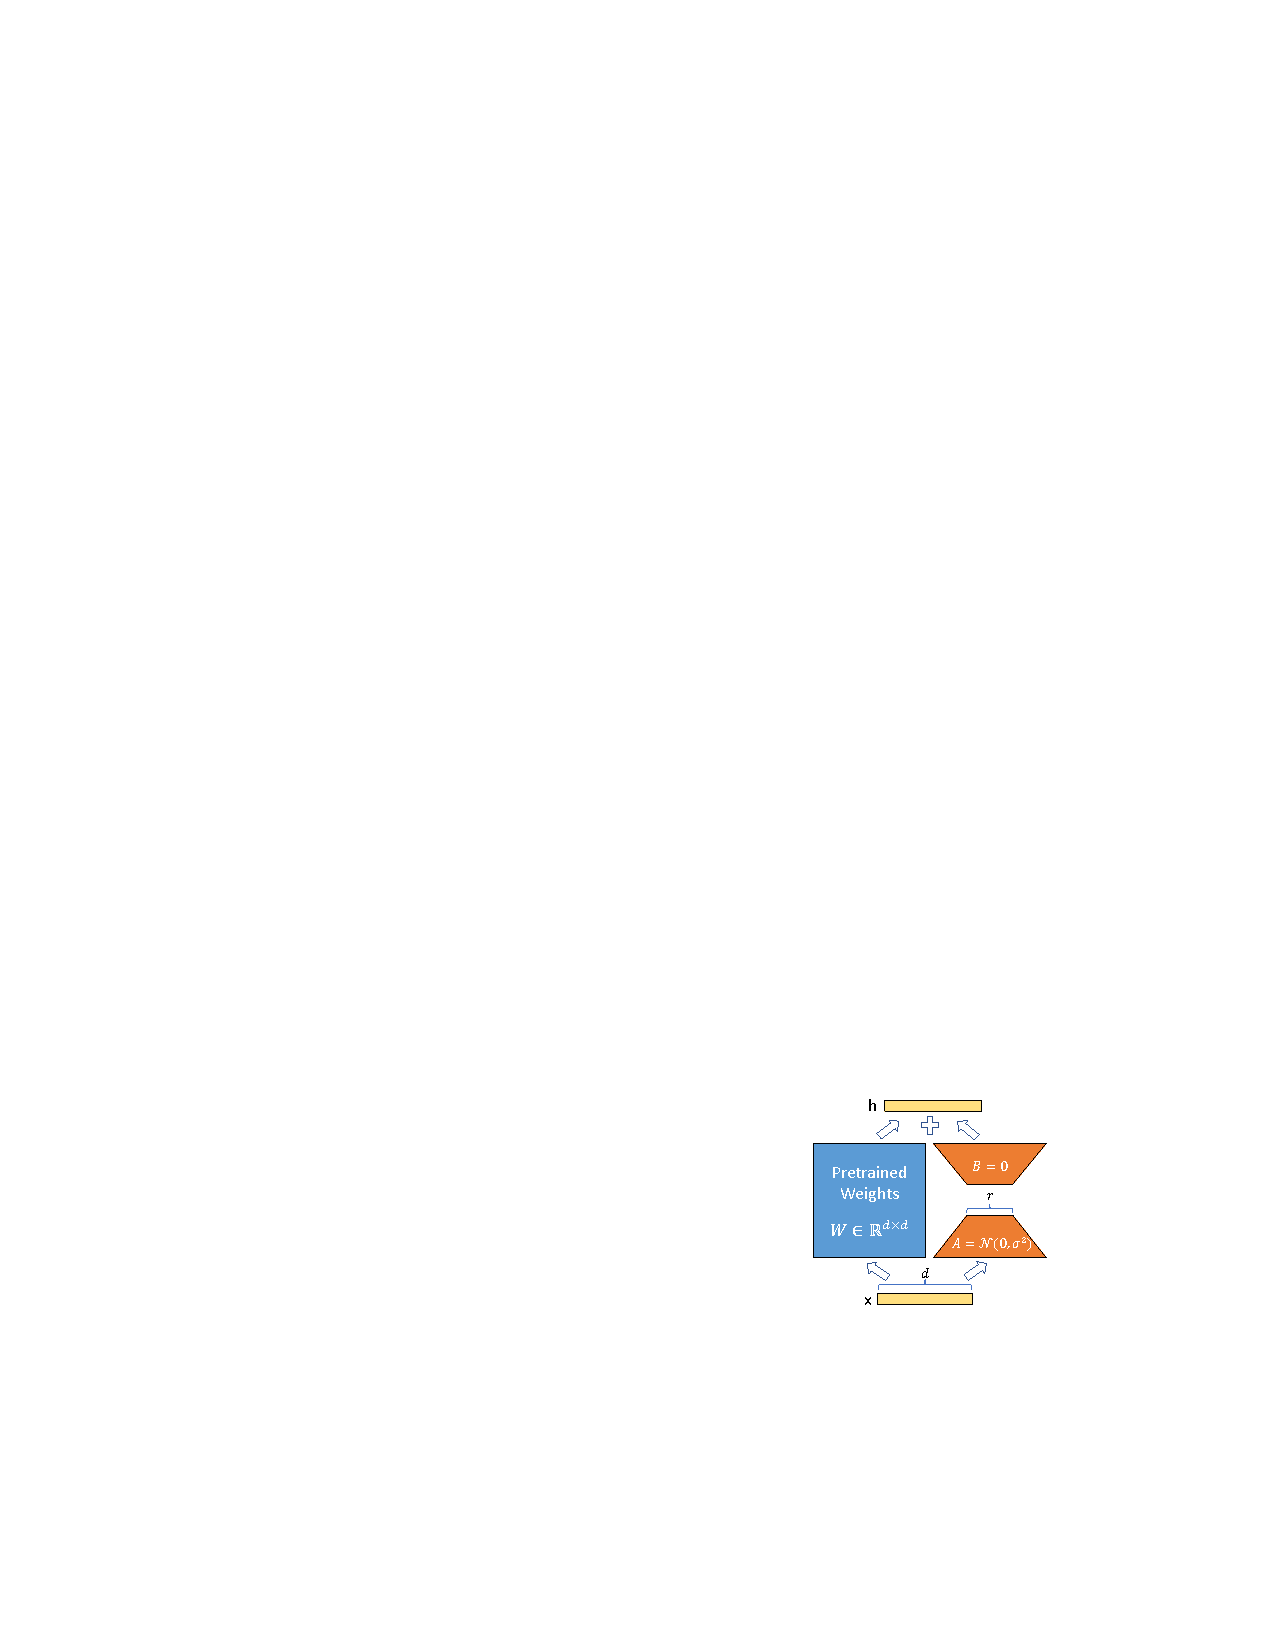
\includegraphics[width=0.5\textwidth]{images/Hu2021_LoraArch.pdf}
    \caption[LoRa Architecture]{LoRa architecture with the docomposed $\Delta W_n = AB$ and their initialization  method (graphic lifted from~\cite{Hu2021})}\label{fig:loraarch}
\end{figure}

\begin{equation}
    W = W_0 + BA
    \label{eq:lora}
\end{equation}

There are more approaches for fine-tuning transformers, which can be explored in further detail in~\cite{Xin2024}.
